\subsection{KNN}
Análisis de KNN
\\
Vamos a analizar el algoritmo KNN (k vecinos mas cercanos) para distintos valores de k, fijando un valor de $\lambda$, para ver como varía la efectividad (cantidad de aciertos) del algoritmo.
Vamos a probar el algoritmo KNN para los siguientes valores:

$\alpha$: 10  y $k$: 1, 5, 20, 50, 250.\\

También vamos a ejecutar para los valores anteriores, 5 pruebas iguales para cada uno, ya que el algoritmo varía la cantidad de aciertos dependiendo de la base de datos que analice y no siempre da el mismo resultado.

Este algoritmo lo que hace es, por cada imágen que queremos averiguar a que dígito pertenece, vectorizarla, restarla a cada uno de los vectores imágen y calcular la norma 2 para saber en cuanto difieren con cada una de las imágenes.
Todos esos resultados los vamos metiendo en una cola de prioridad que los ordena de menor a mayor, según las diferencias entre la imágen que quiero averiguar a que dígito pertenece y todas las imágenes de la base de datos.
\\
Luego lo que hacemos es agarrar los k primeros de la cola de prioridad y verificar a que dígito se corresponden para luego saber cual es el dígito que recibió mas \'votos\' y ver si se produjo un acierto o no.
Por lo tanto, a mayor cantidad de vecinos (o sea, k) menor va a ser la cantidad de aciertos, ya que se empiezan a mirar los elementos de menor prioridad de la cola, eso significa, que se cuentan primero las imágenes que mas difieren y eso puede hacer que las chances de acertar el dígito correcto disminuyan.
\\
El algoritmo $KNN$ es muy efectivo ya que tiene aproximadamente entre 85\% y 90\% de aciertos. Pero su \'déficit\' es que es muy lento a comparación del algoritmo $PCA$. 

\subsubsection{Cantidad de vecinos}
Cantidad de vecinos para el KNN.\\ 
Vamos a analizar para el algoritmo KNN cual es el mejor número de vecinos para el cual da una mayor cantidad de aciertos.
Vamos a probar el algoritmo KNN para los valores siguientes:\\
k: 1, 5, 20, 50, 250.\\

A continuaci\'on vamos a mostrar los resultados para los valores reci\'en mencionados en forma de graficos.

Una de las cosas que podemos observar es que a menor cantidad de vecinos recorridos, mayor va a ser la cantidad de aciertos, ya que como estoy eligiendo los mejores de la cola de prioridad, voy a obtener mayor presici\'on debido a que los primeros de la cola son los que menos difieren de las im\'agenes de la base de datos.
Por lo tanto, si elijo $k = 1$ voy a obtener la im\'agen del d\'igito que m\'as cerca estuvo de la imágen que me pasaron por parámetro, así que no me interesa saber cuales son los resultados de las siguientes imágenes de la cola ya que el primero es el mejor caso posible.



\subsubsection{Mejoras en kNN}
Cortar el dataset en x valor y comparar para ver si mejora

\subsection{PCA}
Vamos a probar el algoritmo para distintas medidas de k y $\alpha$, que van a ser:\\
k: cantidad de vecinos a considerar en el algoritmo $kNN$.\\
$\alpha$: a la cantidad de componentes principales a tomar.

Vamos a probar el algoritmo para los siguientes valores:\\ \\
$\alpha$: 10  y k: 5, 20.\\
$\alpha$: 200 y k: 5, 20.\\
$\alpha$: 700 y k: 5, 20.\\
$\alpha$: 50  y k: 5, 25, 50, 100.\\

Lo que vamos a probar es, fijando un valor de $\lambda$, para que cantidad de vecinos vamos a tener la mayor cantidad de aciertos y así maximizar la cantidad de aciertos.
Después de aplicar el algoritmo $PCA$, aplicamos el $KNN$ y armamos una cola de prioridad para los resultados de aplicar el algoritmo $KNN$. Lo que se hace es tomar dos imágenes, restarlas y aplicarle la norma 2 para saber en cuanto difiere una imágen de la otra. En la cola de prioridad estan adelante los valores más chicos, o sea, las imágenes del test que más cerca de coincidir están con respecto a la imágen de la base de datos.
Por lo tanto, si elegimos una mayor cantidad de vecinos, pueden pasar dos cosas:

\begin{itemize}
  \item Que sea beneficioso ya que a mayor cantidad de pruebas vamos a tener mas aciertos
  \item Que sea malicioso ya que a mayor cantidad de pruebas vamos a obtener peores datos, o sea, vamos a mirar las imagenes que menos coiciden con la imágen de prueba de la base de datos.
\end{itemize}

La conclusión que se desprende es que a mayor cantidad de vecinos, el algoritmo empieza a funcionar peor, ya que estamos mirando los vecinos que menos coinciden con la base de datos, debido a que la cola de prioridad los ordena según la menor cantidad de diferencias entre la imágen obtenida y las imágenes de la base de datos. 

Por lo tanto, cuanto mas vecinos se exploran, menor cantidad de aciertos hay. Eso se puede ver a través de las siguientes mediciones realizadas para distintos $k$ vecinos y fijando un valor de $\lambda$.

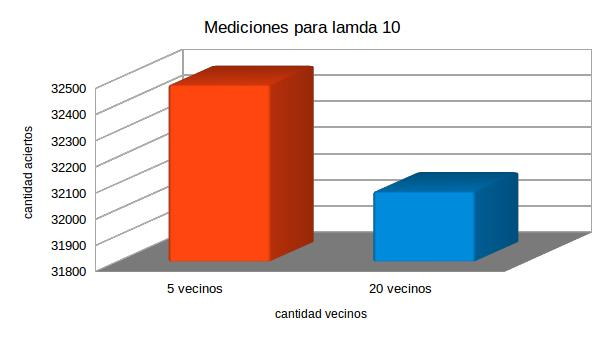
\includegraphics[scale=0.75]{lamda10.jpg}\\
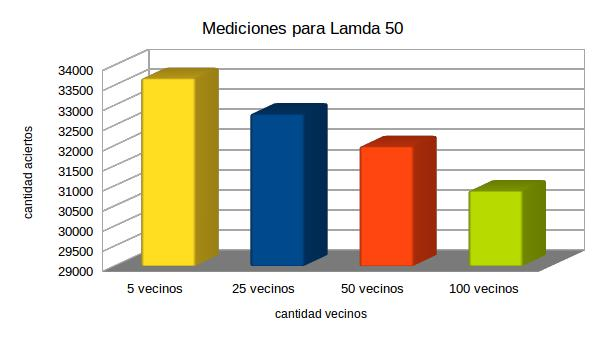
\includegraphics[scale=0.75]{lamda50.jpg}\\
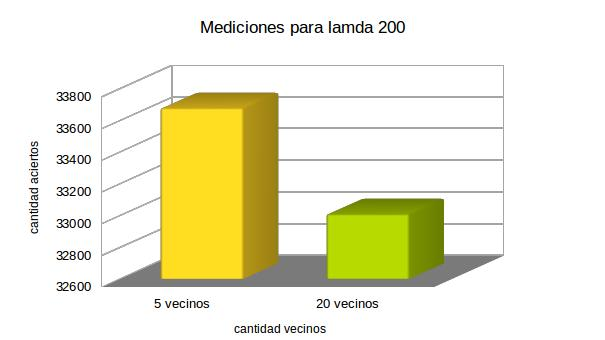
\includegraphics[scale=0.75]{lamda200.jpg}\\
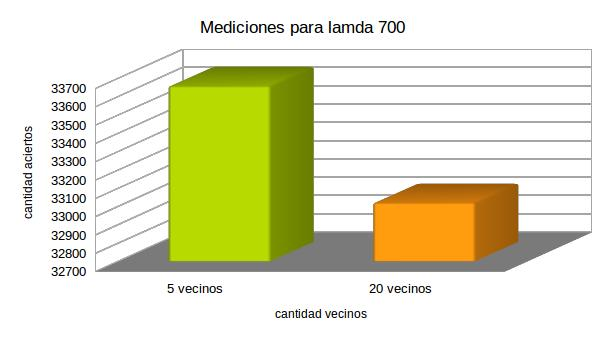
\includegraphics[scale=0.75]{lamda700.jpg}\\

Las pruebas para $\lambda = 10$, $\lambda = 50$ y $\lambda = 200$ las corrimos 10 veces y calculamos un promedio de esas diez. Ese es el valor que se refleja en la cantidad de aciertos. \\

Las pruebas para $\lambda = 700$ las corrimos 4 veces y calculamos un promedio de esas cuatros. Ese es el valor que se refleja en la cantidad de aciertos. \\

Para verificar los datos anteriores, revisar el archivo "mediciones y graficos" en el directorio "informe-resultadostest".



%Otra conclusión que sacamos es que $k = 5$ vecinos es la mejor cantidad de vecinos para obtener la mayor cantidad %de aciertos. 
%Ahora, ¿No sería mejor agarrar solo el primero de la cola de prioridad, es decir, $k = 1$? 
%Lo que podría pasar es que el único vecino que utilicemos sea el mejor pero no alcance para saber cuál es el %dígito de la imagen, ya que si no se acierta con el único vecino que se elije,  podría fallar el dígito del %resultado, reduciendo en un alto grado la cantidad de aciertos.

\subsubsection{Lambda inicial}

\subsubsection{Algo más que no me acuerde}
